\chapter{Alignment Procedure}
\label{ch:howtoalign}

This chapter provides a description of how to use the alignment features of \corry. 
It also includes step-by-step instructions on how to align a new set of testbeam data.

For the alignment of the \textbf{reference telescope} and \textbf{device-under-test (DUT)}, the following modules are available in \corry (see also \ref{ch:modules}).
\begin{itemize}
\item \texttt{Prealignment} for both telescope and DUT prealignment (see also \ref{prealignment}).
\item \texttt{AlignmentTrackChi2} used for telescope alignment (see also \ref{alignmenttrackchi2}).
\item \texttt{AlignmentDUTResidual} used for DUT alignment (see also \ref{alignmentdutresidual}).
\item \texttt{AlignmentMillepede} for an improved telescope alignment (see also \ref{alignmentmillepede}).
\end{itemize}

Scripts to run and configure \corry should be stored in a separate git repository as they do not belong directly to the \corry framework and are highly user-specific.
Working examples can be found here: \texttt{path/to/corryvreckan/\textbf{testing/}}.

It contains the subdirectory \texttt{geometries/} with all the detector files which provide detector and alignment information.
It also contains the scripts that are run to call and configure \corry for alignment and analysis.
The user is welcome to modify these configuration files and play with the applied cuts etc. to get a better understanding of \corry.

\textbf{Note:} \corry can handle any file extensions for geometry and configuration files. The examples, however, follow the convention of using the extension \texttt{*.conf} for both detector and configuration files.

The general procedure that needs to be followed for a sucessful alignment is outlined here and explained in detail below.
\begin{enumerate}
\item prealign telescope (ignore DUT)
\item align telescope (ignore DUT)
\item prealign DUT (telescope geometry is frozen)
\item align DUT (telescope alignment is frozen)
\end{enumerate}

\textbf{Note:} When using the alignment modules, the new geometry is written out to a new geometry file which needs to be specified using the parameter \texttt{detectors\_file\_updated}.
It can be the same as the input \texttt{detectors\_file} causing it to be overwritten.
However, this is not recommended.

\section{Aligning the Telescope}
\label{sec:align_tel}
To begin with, the telescope needs to be aligned. 
For this, the DUT is completely ignored.

\subsection*{Prealignment of the Telescope}
The \texttt{AlignmentTrackChi2} module requires a careful prealignment. Otherwise it does not converge and the alignment will fail.
For the prealignment, two tricks can be played.
\begin{itemize}
\item A rough manual prealignment can be performed by having a look at correlations plots between a defined reference plane and the others planes in both x and y.
These can be found in the module \texttt{TestAlgorithm}.
\item The \texttt{Prealignment} module can be used.
\end{itemize}

The z-position of all planes needs to be measured by hand in the existing testbeam setup and then adjusted in the detectors file. 
It will not be changed during the alignment process.
For x and y, the alignment file from the last testbeam is a solid basis to start from.
If no previous alignment is available, all values for x and y should be set to 0.

To have a first look at the initial alignment guess, one can run
\begin{verbatim}
    /path/to/corryvreckan/bin/corry 
        -c analyse_telescope.conf
    	[-o detectors_file=<detectorsFile> 
    	-o histogramFile=<histogramFile> 
    	-o EventLoaderTimepix3.inputDirectory=<inputDir>]
\end{verbatim}

The \texttt{spatialCut} in \texttt{[Tracking4D]} should be set to mulitple ($\sim4$) pixel size.

One can inspect the track $\chi^2$, the correlation in x and y and the residuals with the online monitoring or by opening the generated ROOT file after finishing the script (see \texttt{[Tracking4D]} and \texttt{[TestAlgorithm]}).

\textbf{Tip:} To save time, one can terminate \corry with \texttt{Ctrl+C} after a while (see also \ref{sec:executable}).

If no peak at all is apparent in the correlations, the hitmaps can be checked to see if valid data is actually available for all planes.

For the residuals, the shift of the peak from 0 can be estimated with a precision of $\mathcal{O}(\SI{100}{\micro m})$ by zooming in using the \texttt{TBrowser}.
For instance, if the peak is shifted by +\SI{+300}{\micro m}, the detectors file needs to be edited and \SI{+300}{\micro m} should be added to the respective position, if \SI{-300}{\micro m}, subtracted.

After modifying the positions of individual planes in the configuration file, \corry can be re-run to check the correlation plots for the updated geometry.
These steps need to be iterated a few times until the peaks of the \textit{residuals} are centered around 0.
 
It is important not to force the peak of the \textit{correlations} to be at exactly 0 because the position of the peak in fact corresponds to the physical offset of a plane from its ideal position. 

Instead of a prealignment by hand, the \texttt{Prealignment} module can be used.
It is a \textit{DETECTOR} type module so it is instantiated once for each plane (including DUTs).
To prealign only the telescope, the DUT can be masked by setting \texttt{mask = <name\_of\_dut>}.
However, all planes can be prealigned at once.

Since the prealignment utilizes hit correlations rather than tracks, no cuts are needed here.

To use the module, \texttt{align\_tel.conf} needs to be edited such that \texttt{Prealignment} is enabled and \texttt{Alignment} is disabled:
\begin{minted}[frame=single,framesep=3pt,breaklines=true,tabsize=2,linenos]{ini}
...
[Prealignment]
mask = <name_of_dut> # <-- optional!
[Ignore]
#[AlignmentTrackChi2]
log_level=INFO
iterations = 4
alignOrientation=true
alignPosition=true
\end{minted}

Then one can run
\begin{verbatim}
    /path/to/corryvreckan/bin/corry 
        -c align_telescope.conf
    	[-o detectors_file=<detectorsFile> 
    	-o detectors_file_updated=<detectorsFileUpdated> 
    	-o histogramFile=<histogramFile> 
    	-o EventLoaderTimepix3.inputDirectory=<inputDir>]
\end{verbatim}

The actual prealignment is only performed after the events have been analysed and written to the detectors file in the finalizing step. 
This means to check whether the alignment has improved, one needs to re-run the analysis or the next iteration of the alignment as the previously generated ROOT file corresponds to the alignment you started from.
This is the case for every iteration of the prealignment or alignment.

Generally, it suffices to run the \texttt{[Prealignment]} module once and then proceed with the next step.

\subsection*{Alignment of the Telescope}
After the prealignment, the actual \textit{precise} alignment can be performed using the \texttt{AlignmentTrackChi2} module.
To this end, \texttt{align\_tel.conf} needs to be modified such that the prealignment is disabled and the alignment is enabled:
\begin{minted}[frame=single,framesep=3pt,breaklines=true,tabsize=2,linenos]{ini}
...
#[Prealignment]
#[Ignore]
[AlignmentTrackChi2]
log_level=INFO
iterations = 4
alignOrientation=true
alignPosition=true
\end{minted}

The algorithm performs an optimisation of the track $\chi^2$.
Typically, the alignment needs to be iterated a handful of times until the residuals (which again can be inspected in the ROOT file after re-running the analysis) are nicely centered around 0 and narrow.
In fact, the width of the residuals corresponds to the spatial resolution of each plane and should thus be smaller than the respective pixel size.
Starting with a \texttt{spatialCut} in \texttt{[Tracking4D]} of multiple ($\sim4$) pixel sizes, it should be decreased incrementally down to the pixel size (e.g. run \SI{200}{\micro\m} twice, then run \SI{150}{\micro\m} twice, then \SI{100}{\micro\m} twice, and then \SI{50}{\micro\m}) twice.
This allows to perform the alignment with a tight selection of very high quality tracks only.
Also the \texttt{max\_track\_chi2ndof} should be decrease for the same reason.
For the further analysis, the cuts can be released again.

Sometimes, the procedure runs into a 'false minimum' or 'gets stuck' and does not converge properly which requires to go one step back and improve the prealignment.

Once the alignment is done, one should obtain narrow residuals centered around 0 and a good distribution of the track $\chi^2$ as shown in Figures~\ref{fig:exampleAlignment}.
If the alignment keeps to fail, it is possible to allow only for rotational or translational alignment while freezing the other for one or a few iterations.

\begin{figure}
    \centering
    \begin{subfigure}[t]{0.66\textwidth}
        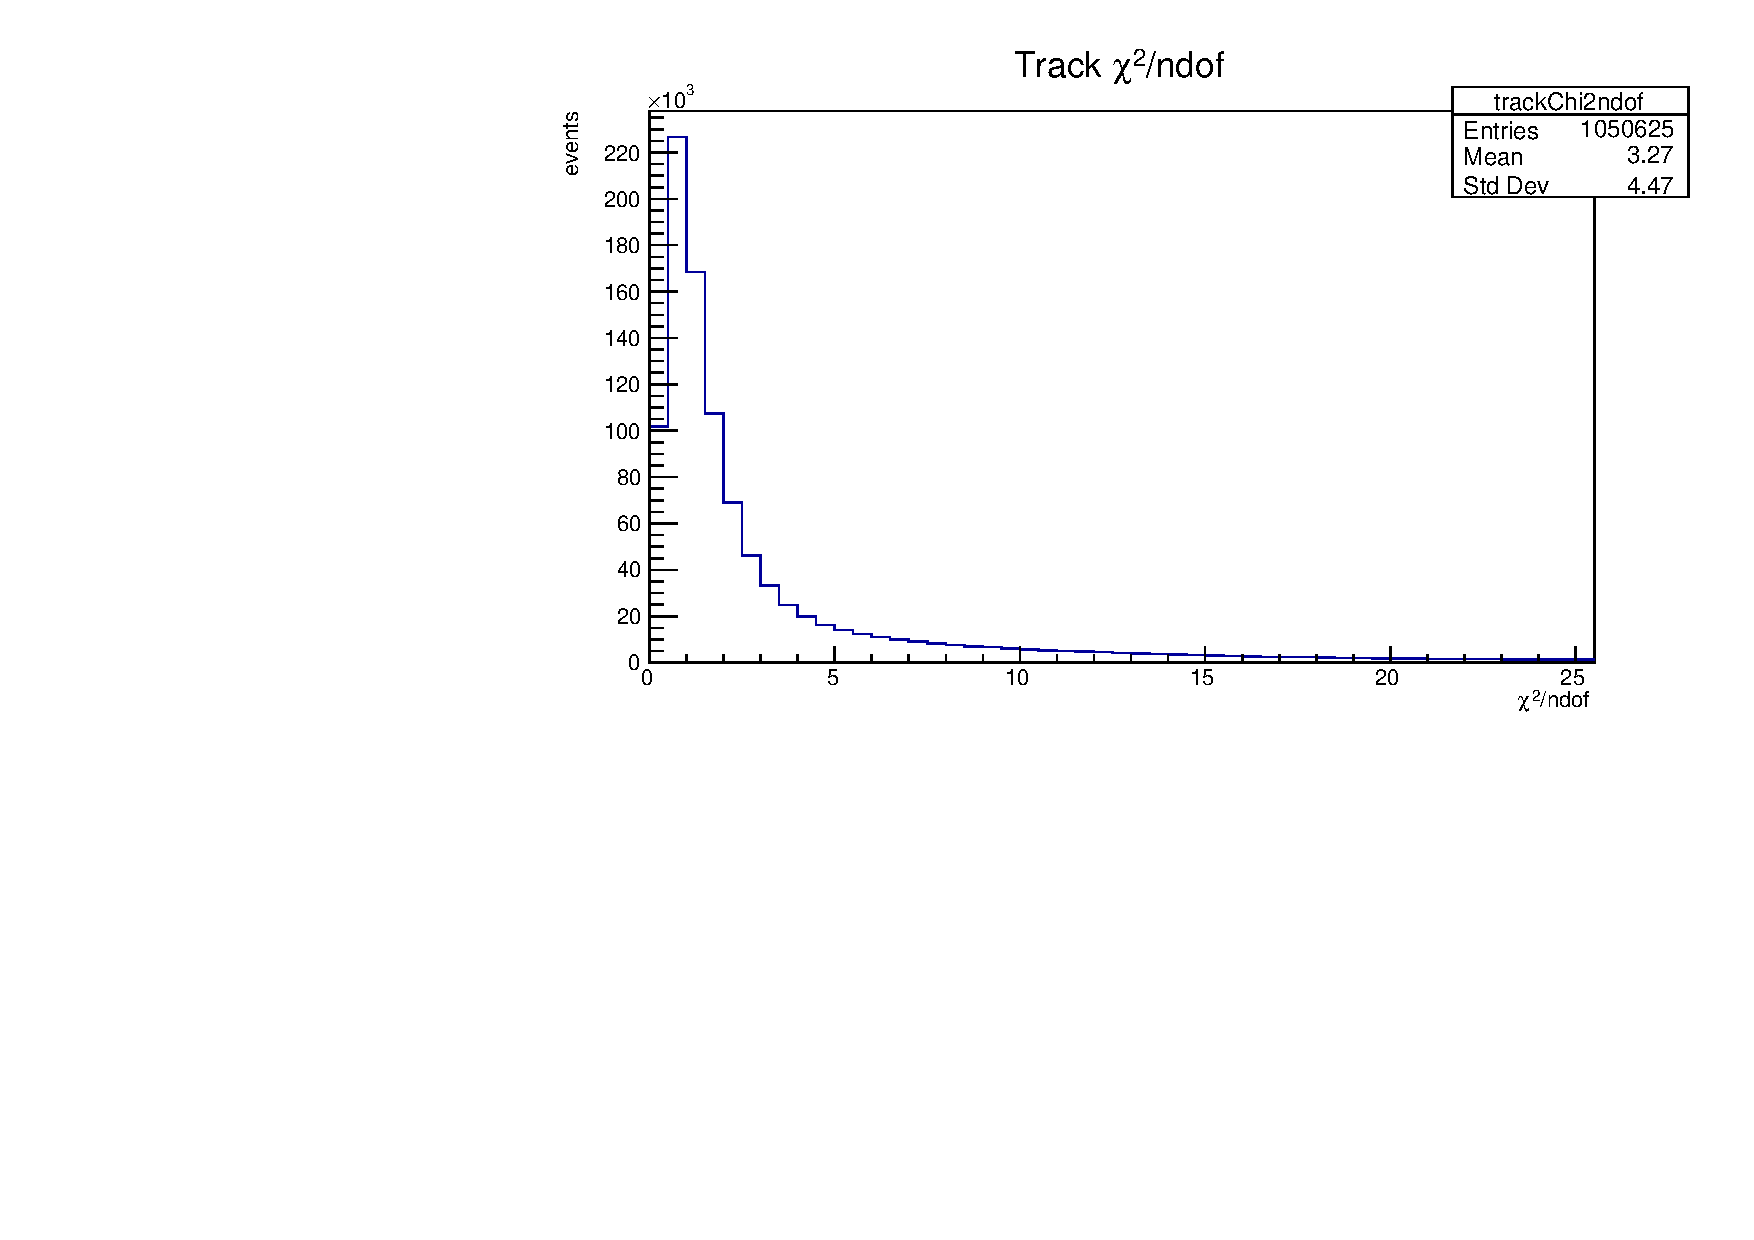
\includegraphics[width=\textwidth]{trackChi2ndof_goodexample}
        \caption{Good example of a track $\chi^2$/ndf distribution.}
        \label{fig:trackChi2}
    \end{subfigure}
    \begin{subfigure}[t]{0.66\textwidth}
        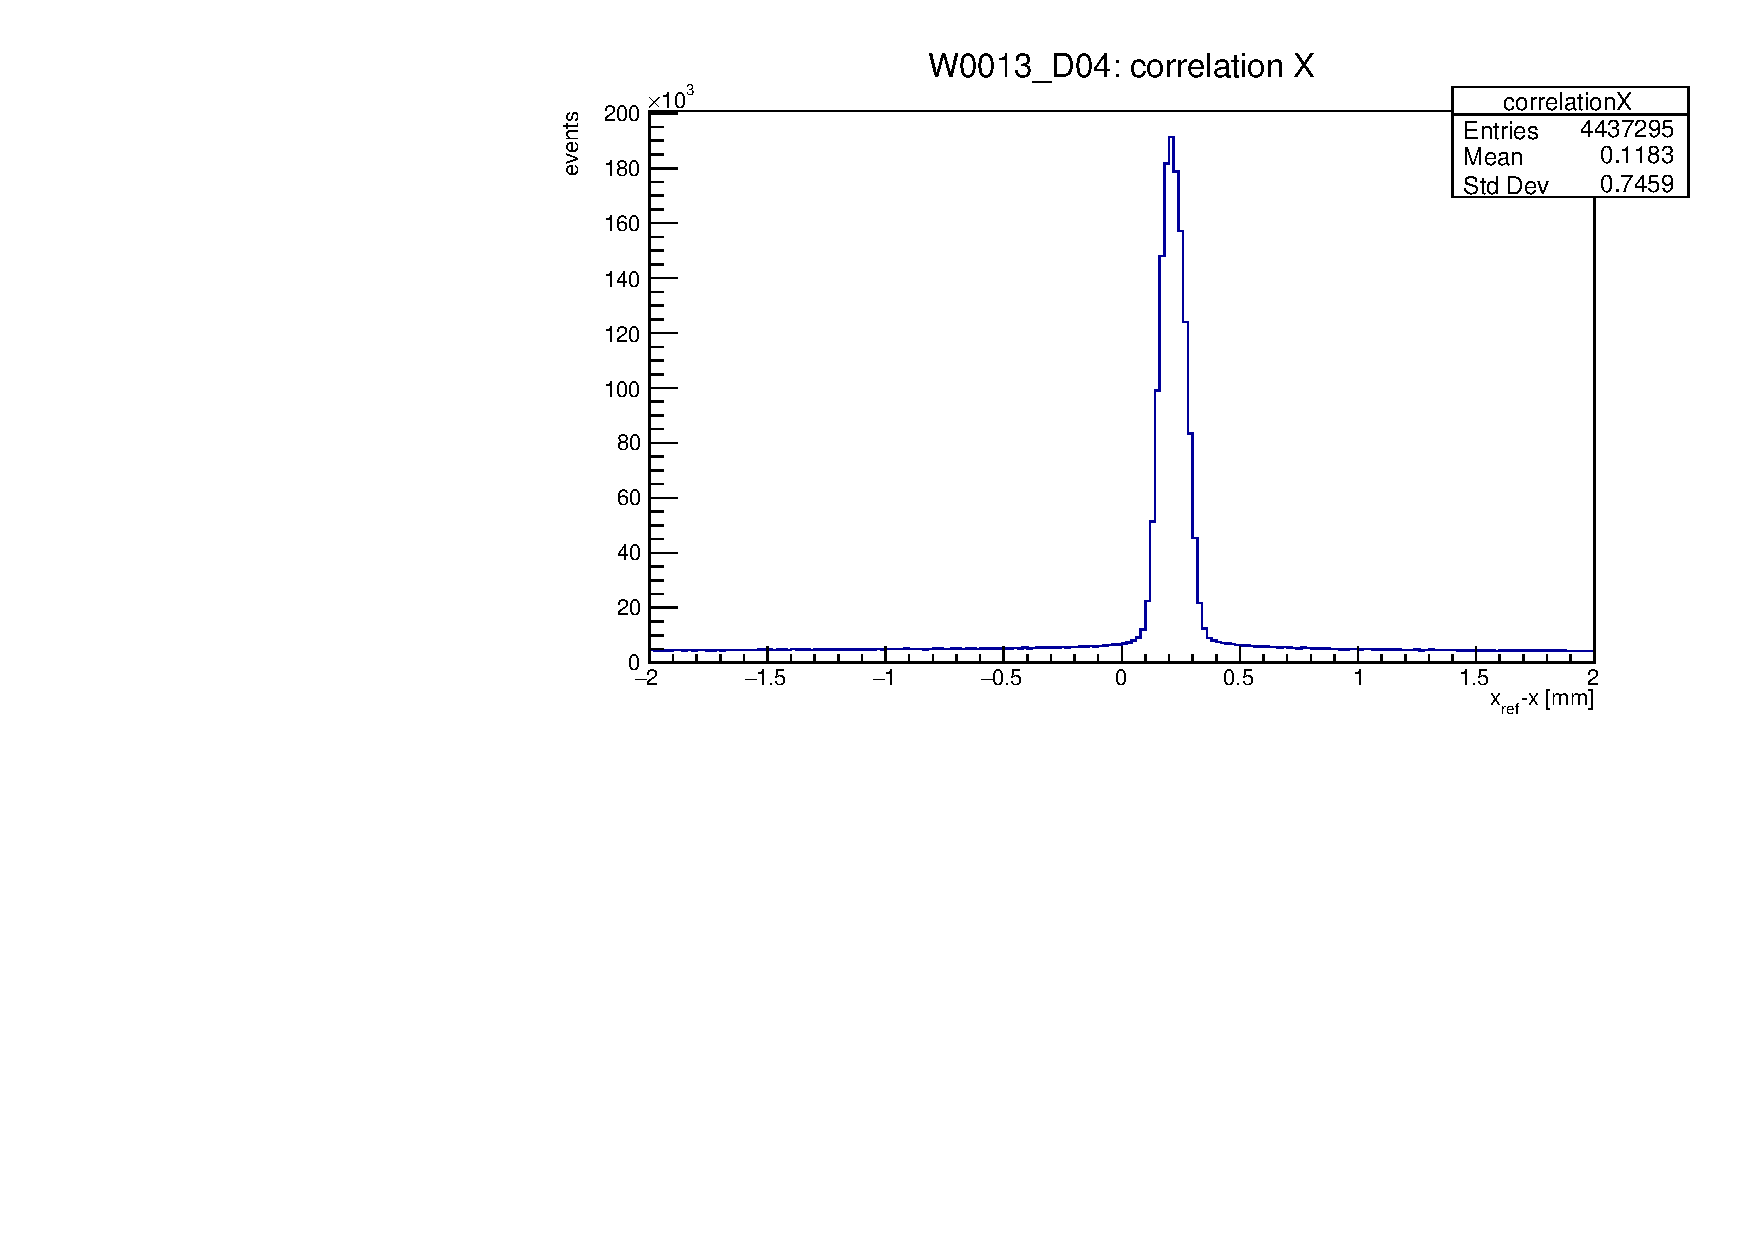
\includegraphics[width=\textwidth]{correlationX_goodexample}
        \caption{Good example of a correlation plot.}
        \label{fig:correlationX}
    \end{subfigure}
    \begin{subfigure}[t]{0.66\textwidth}
        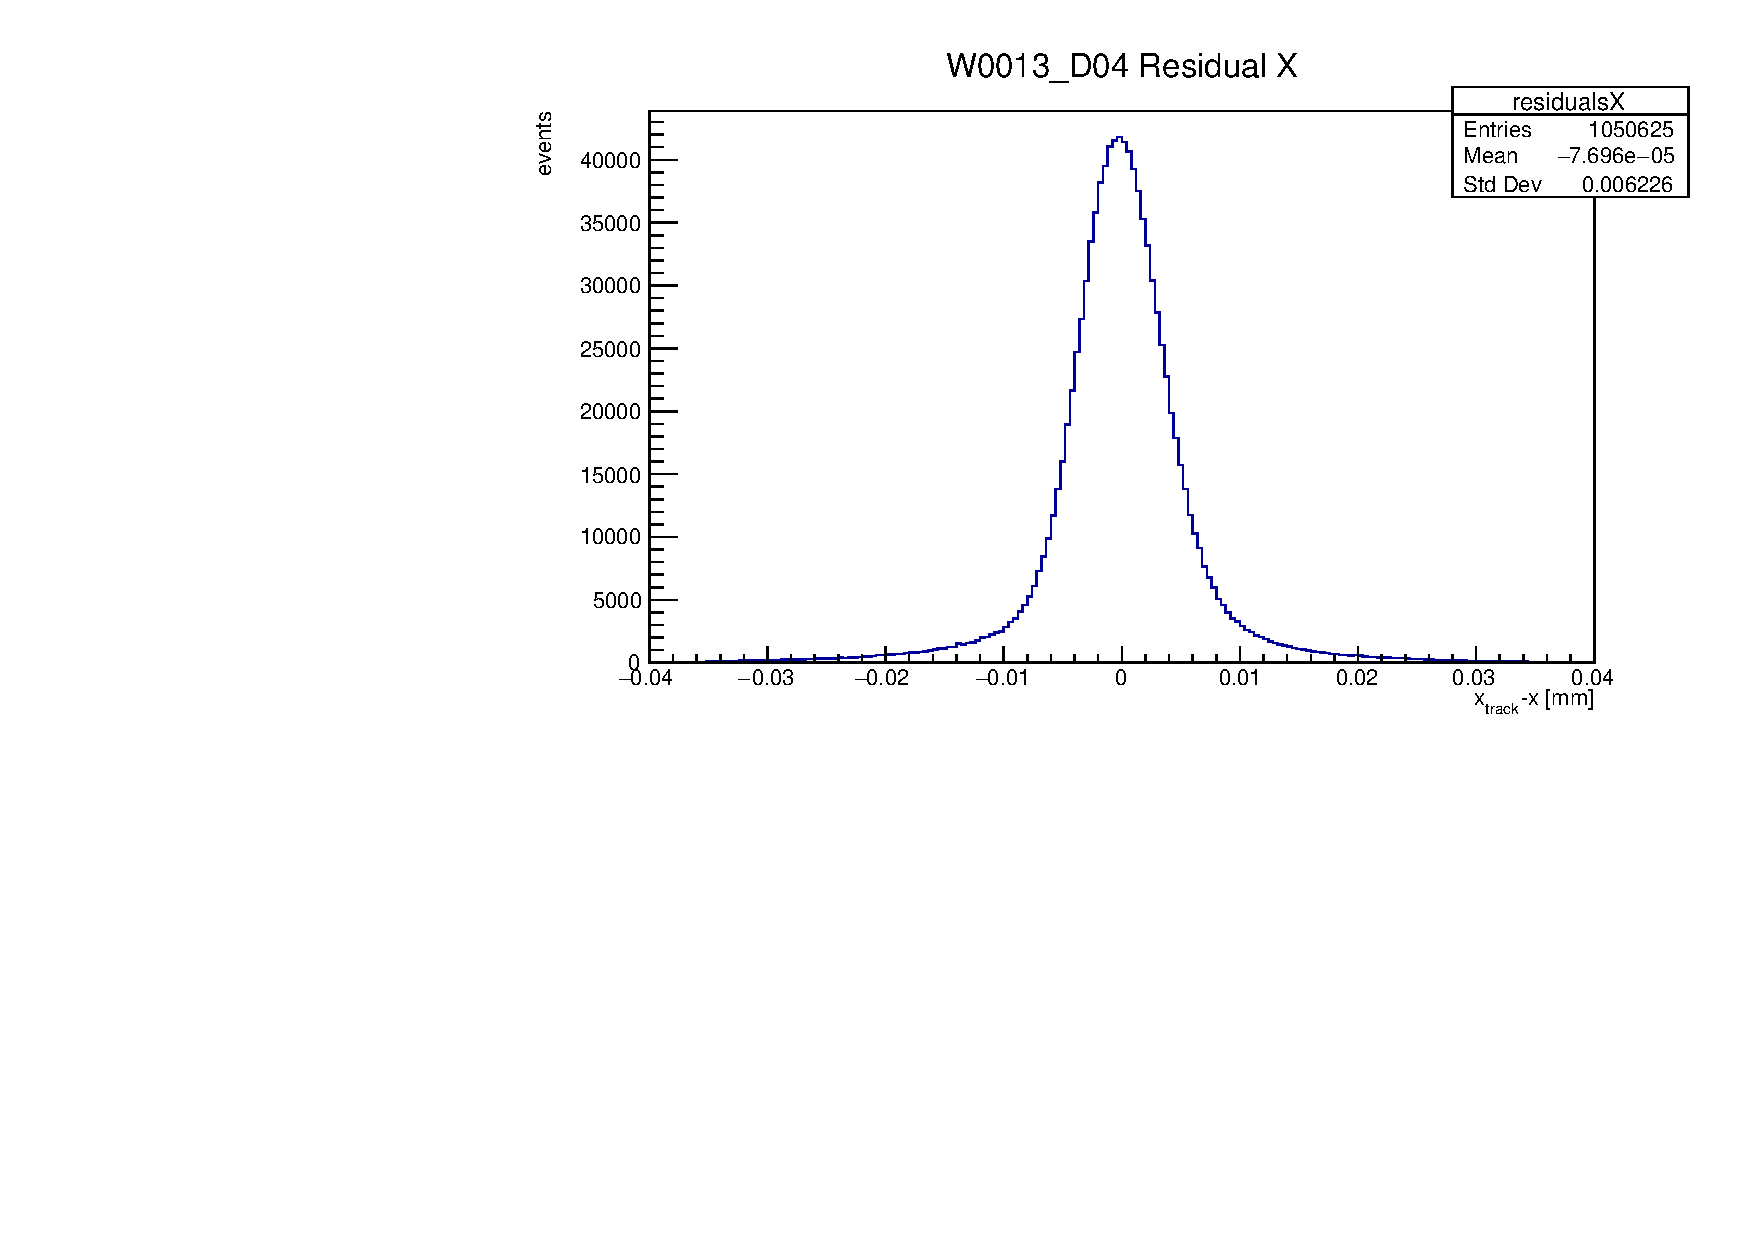
\includegraphics[width=\textwidth]{residualX_goodexample}
        \caption{Good example of a residual distribution.}
        \label{fig:residualX}
    \end{subfigure}
    \caption{Examples of distributions as they should look like.}
    \label{fig:exampleAlignment}
\end{figure}

\textbf{Note:} When starting the alignment procedure from a slightly different initial geometry, the resulting alignment (i.e.~the numbers in the detectors file) will differ slightly which is acceptable. What should \textbf{not} differ is the width of the residuals.

\section{Aligning the DUT}
\label{sec:align_dut}
Once the telescope is aligned, its geometry is not touched anymore. From now on, it is used to build tracks which are then matched to clusters on the DUT.

\subsection*{Prealignment of the DUT}
The prealignment of the DUT follows the same strategy as for the telescope. To look at the current alignment, the script
\begin{verbatim}
    /path/to/corryvreckan/bin/corry 
    	-c analyse_atlaspix.conf 
    	[-o detectors_file=<detectorsFile> 
    	-o histogramFile=<histogramFile> 
    	-o EventLoaderTimepix3.inputDirectory=<inputDir_TPX>
    	-o EventLoaderATLASpix.inputDirectory=<inputDir_APX>]
\end{verbatim}
needs to be run.
If no better guess is available, the initial alignment of the DUT should be set to $x=y=z=0$.

Then, by repeatedly running \corry and modifying the position of the DUT in the detectors file one should be able to bring the peaks of the correlations in x and y close to 0.
If no peak at all can be seen in the correlation plots, potentially some values need to be corrected in the configuration file.
If working with an ATLASpix, these are most likely \texttt{clockCycle} or \texttt{clkdivend2} in \texttt{[EventLoaderATLASpix]}.

\textbf{Important: }If using the \texttt{[Prealignment]} module, it is possible to prealign all planes at once as described above.
If only the DUT shall be prealigned here, the parameter \texttt{name = <name\_of\_dut>} needs to be used.
Otherwise, the telescope planes are also shifted again destroying the telescope alignment.

\begin{minted}[frame=single,framesep=3pt,breaklines=true,tabsize=2,linenos]{ini}
...
[Prealignment]
name = <name_of_dut> # <-- otherwise telescope planes will be moved!

[Ignore]
#[AlignmentDUTResiduals]
log_level=INFO
iterations = 4
alignOrientation=true
alignPosition=true
\end{minted}

\subsection*{Alignment of the DUT}
Again, the alignment strategy for the DUT is similar as for the telescope and requires multiple iterations.
In \texttt{align\_dut.conf}, the prealignment needs to be disabled and the alignment enabled.
Now, the algorithm optimizes the residuals of the tracks through the DUT.

\begin{minted}[frame=single,framesep=3pt,breaklines=true,tabsize=2,linenos]{ini}
...
#[Prealignment]
#[Ignore]
[AlignmentDUTResiduals]
log_level=INFO
iterations = 4
alignOrientation=true
alignPosition=true
\end{minted}

Then run
\begin{verbatim}
    /path/to/corryvreckan/bin/corry 
    	-c align_dut.conf 
    	[-o detectors_file=<detectorsFile> 
    	-o detectors_file_updated=<detectorsFileUpdated> 
    	-o histogramFile=<histogramFile> 
    	-o EventLoaderTimepix3.inputDirectory=<inputDir_TPX>
    	-o EventLoaderATLASpix.inputDirectory=<inputDir_APX>]
\end{verbatim}

\textbf{Note:} The histograms of the residuals for the DUT in \texttt{[Tracking4D]} are empty. The correct ones can be found in \texttt{[AnalysisDUT]}.

Like for the telescope alignment, the widths of the residuals can be interpreted as the spatial resolution of the DUT and should should thus be $\lesssim$~pixel size.
Again, starting with a \texttt{spatialCut} in \texttt{[DUTAssociation]} of multiple ($\sim4$) pixel sizes, it should be decreased incrementally down to the pixel size. Note that an asymmetric pixel geometry requires the \texttt{spatialCut} to be chosen accordingly.

If the alignment keeps to fail, it is possible to allow only for rotational or translational alignment while freezing the other for one or a few iterations.

\begin{minted}[frame=single,framesep=3pt,breaklines=true,tabsize=2,linenos]{ini}
...
#[Prealignment]
#[Ignore]
[AlignmentDUTResiduals]
log_level=INFO
iterations = 4
alignOrientation=false #<-- disable rotational alignment
alignPosition=true
\end{minted}

\section{FAQs and Special Remarks}
Here a common problems and solutions are/will be described.
Suggestions are welcome.
\begin{itemize}
\item add any problem and solution here
\end{itemize}
